%! Author = adnansiddiquei
%! Date = 13/12/2023

\subsection{Dataset A}\label{sec:dataset-a}
    \begin{figure}[htb]
    \centering
    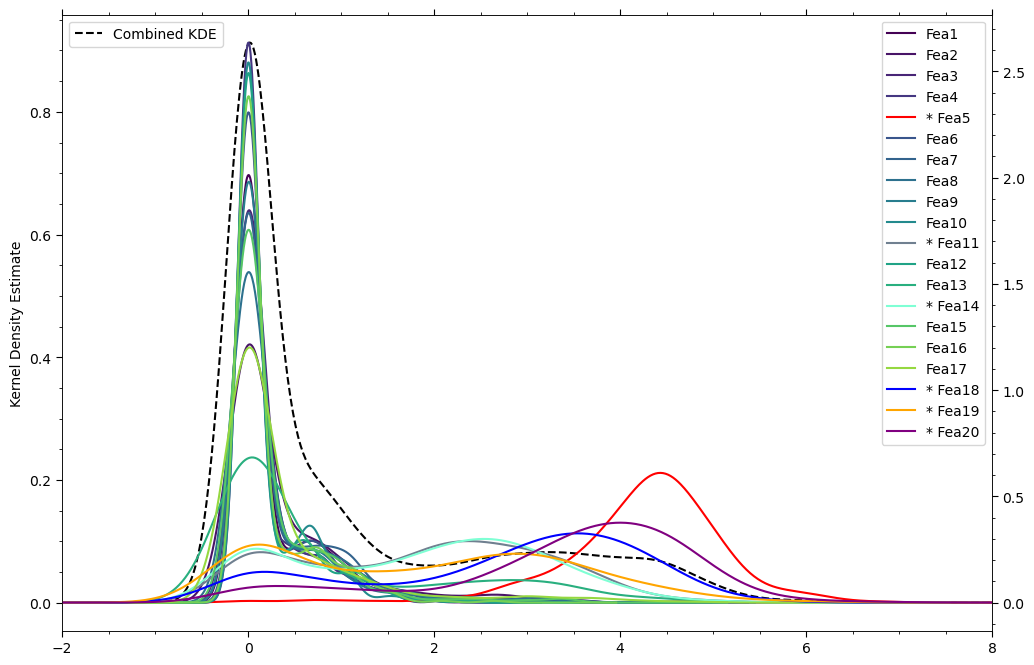
\includegraphics[width=0.9\textwidth]{./figures/q1a}
    \caption{A kernel density estimate of the first 20 features of the dataset, which has 20 plots in total, with the
    legend and corresponding y-axis on the right. A combined KDE has also been plotted, with it's corresponding x-axis
    on the left. 6 of the 20 features have been highlighted in the legend with an asterisk, and have been coloured in
    slightly more contrasting colours to highlight them. These features contain more density in the non-zero region
    and are likely to be more discriminative.}
    \label{fig:q1a}
    \end{figure}

    Fig\ref{fig:q1a} shows the combined and separated kernal density estimates of the first 20 features of the dataset.
    Several conclusions can be drawn from this plot.
    For most of the features, the KDE is concentrated around the zero value, with the exception of features 5, 11, 14,
    18, 19 and 20.
    These features are likely to be more discriminative, as they contain more variability.
    Feature 5 is concentrated around a value of 4.5, whilst the other 5 of these discriminative features are more widely
    spread around the range of values, which gives them more potential to be more discriminative in classification
    algorithms.
